Das Thema \emph{soziale Netzwerke} wurde in den letzten Jahren immer
popul\"arer. Wie man in Abbildung~\ref{fig:overall} sieht, waren es im Jahr
2010 lediglich knapp eine Milliarde Nutzer weltweit, die sich in solchen
Netzwerken angemeldet hatten. Die Zahl stieg stetig an. Innerhalb von f\"unf
Jahren (2015) hat sich diese Anzahl mehr als verdoppelt auf $2,14$ Milliarden
Nutzer. Das stetige Wachstum wird auch f\"ur die Zukunft prognostiziert.
\begin{figure}[ht]
	\centering
	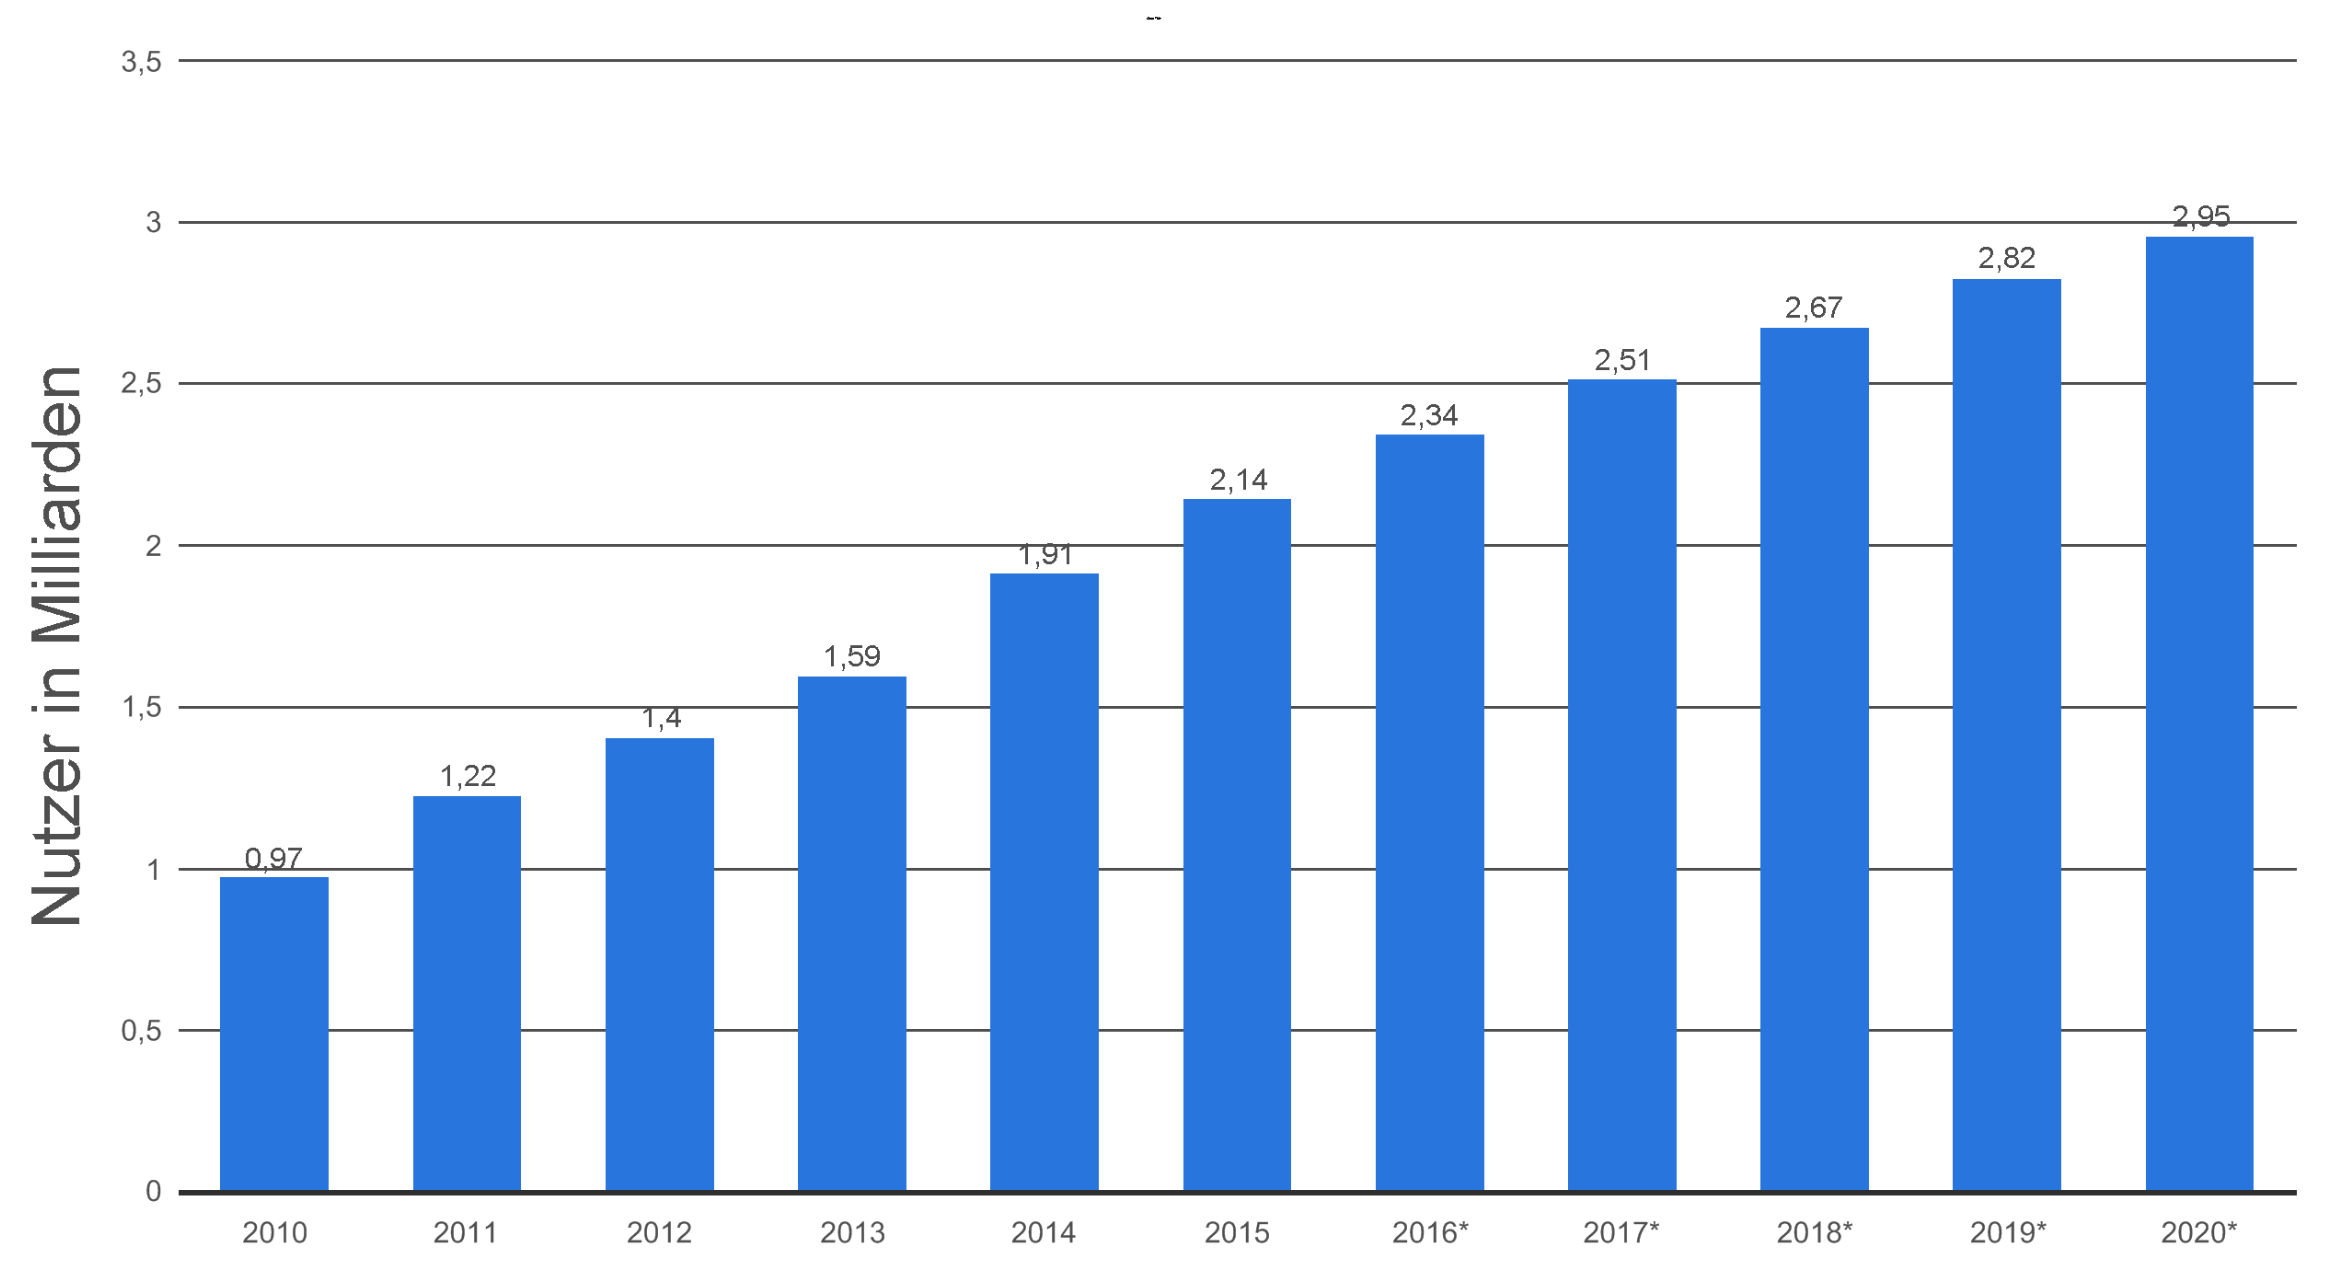
\includegraphics[scale=0.6]{resources/einf_02.png}
	\caption{Anzahl der Nutzer sozialer Netzwerke weltweit in den Jahren 2010
	bis 2015 sowie eine Prognose bis 2020 (in Milliarden)~\cite{statista-allg}.}
	\label{fig:overall}
\end{figure}

Durch die hohe Beliebtheit und vor allem durch den Durchbruch der Smartphones,
sind soziale Netzwerke im allt\"aglichen Leben kaum mehr wegzudenken. Auch
Kinder und Jungendliche kommen immer h\"aufiger und immer fr\"uher in Kontakt
mit diesen Medien~\cite{statista-jugendliche}. Im Jahr 2014 gaben
beispielsweise $72$ Prozent der Kinder und Jugendlichen von $10$ bis $18$
Jahren an, \emph{Whatsapp} aktiv zu nutze. $56$ Prozent der Befragten benutzen
das soziale Netzwerk \emph{Facebook} aktiv~\cite{statista-jugendliche}.


YouNow\footnote{\url{https://www.younow.com}} und
SnapChat\footnote{\url{https://www.snapchat.com}} sind zwei aufstrebende,
neuere Anwendungen in diesem Bereich und vor allem bei Kindern und Jugendlichen
sehr beliebt~\cite{statista-snapchat, vaterlaus2016snapchat}. Im Rahmen dieser
Arbeit werden beide Applikationen n\"aher betrachtet und auf m\"ogliche
Gefahren und vor allem in Bezug auf P\"adophilie untersucht.
